 
% Copyright 2004 by Till Tantau <tantau@users.sourceforge.net>.
%
% In principle, this file can be redistributed and/or modified under
% the terms of the GNU Public License, version 2.
%
% However, this file is supposed to be a template to be modified
% for your own needs. For this reason, if you use this file as a
% template and not specifically distribute it as part of a another
% package/program, I grant the extra permission to freely copy and
% modify this file as you see fit and even to delete this copyright
% notice. 
\AtBeginDocument{\renewcommand{\bibname}{References}}

\documentclass{beamer}
%\usepackage[table]{xcolor}
\usepackage[absolute,overlay,showboxes]{textpos}
\usepackage{caption}
\usepackage{xcolor,colortbl}
\usepackage{amsmath}
%\usepackage{lipsum}
%\AtBeginDocument{\renewcommand{\bibname}{References}}

% There are many different themes available for Beamer. A comprehensive
% list with examples is given here:
% http://deic.uab.es/~iblanes/beamer_gallery/index_by_theme.html
% You can uncomment the themes below if you would like to use a different
% one:
%\usetheme{AnnArbor}
%\usetheme{Antibes}
%\usetheme{Bergen}
%\usetheme{Berkeley}
%\usetheme{Berlin}
%\usetheme{Boadilla}
%\usetheme{boxes}
%\usetheme{CambridgeUS}
%\usetheme{Copenhagen}
%\usetheme{Darmstadt}
\usetheme{default}
%\usetheme{Frankfurt}
%\usetheme{Goettingen}
%\usetheme{Hannover}
%\usetheme{Ilmenau}
%\usetheme{JuanLesPins}
%\usetheme{Luebeck}
%\usetheme{Madrid}
%\usetheme{Malmoe}
%\usetheme{Marburg}
%\usetheme{Montpellier}
%\usetheme{PaloAlto}
%\usetheme{Pittsburgh}
%\usetheme{Rochester}
%\usetheme{Singapore}
%\usetheme{Szeged}
%\usetheme{Warsaw}

\title{Uplink User-Assisted Relaying in Cellular Networks}

% A subtitle is optional and this may be deleted
%\subtitle{Dual Degree Phase 1 Presentation}

\author{Presented by: Prudhvi Porandla \\ \quad (110070039)\\
\vspace{2mm}
Guide: Prof. Prasanna Chaporkar \\
\vspace{2mm}
SRE Presentation}
% - Give the names in the same order as the appear in the paper.
% - Use the \inst{?} command only if the authors have different
%   affiliation.

% - Use the \inst command only if there are several affiliations.
% - Keep it simple, no one is interested in your street address.

%\date{2nd May 2016}
% - Either use conference name or its abbreviation.
% - Not really informative to the audience, more for people (including
%   yourself) who are reading the slides online

%%%%%\subject{Theoretical Computer Science}
% This is only inserted into the PDF information catalog. Can be left
% out. 

% If you have a file called "university-logo-filename.xxx", where xxx
% is a graphic format that can be processed by latex or pdflatex,
% resp., then you can add a logo as follows:

% \pgfdeclareimage[height=0.5cm]{university-logo}{university-logo-filename}
% \logo{\pgfuseimage{university-logo}}

% Delete this, if you do not want the table of contents to pop up at
% the beginning of each subsection:


% Let's get started
\begin{document}

\begin{frame}
  \titlepage
\end{frame}

\begin{frame}{Overview}
  \begin{itemize}
  \item Introduction
  \vspace{3mm}
  \item  Partial Decode-and-Forward Relaying
  \vspace{3mm}
  \item PDF in Cellular Networks
  \vspace{3mm}
  \item Cooperation Policies 
  \vspace{3mm}
  \item Simulations and Results
  \vspace{3mm}
  \item Future Work
  \end{itemize}
  % You might wish to add the option [pausesections]
\end{frame}

% Section and subsections will appear in the presentation overview
% and table of contents.



\begin{frame}{Introduction}
  \begin{itemize}
  \item Relaying cooperative communications will play important roles in future generations wireless networks.
  \vspace{0.5cm}
  \item Relay-aided cooperative communication techniques represent a promising technology that improves average rate
  \vspace{0.5cm}
  \item We use Partial Decode-and-Forward relaying scheme 
  \vspace{0.5cm}
  \item We will explore two policies by which active User Equipments(UEs) pick their relays
  \end{itemize}
  % You might wish to add the option [pausesections]
\end{frame}
%%%%\section{Second Main Section}

\begin{frame}{Partial Decode-and-Forward Relaying} {Two Phases}
Total transmission period is divided into phases: 1. Broadcast phase and 2. Multicast phase as shown in the figure below.
\begin{figure}
\centering
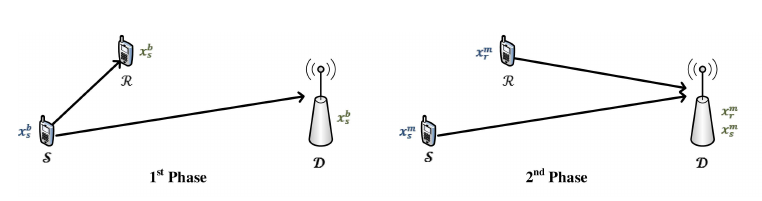
\includegraphics[width=\textwidth]{figures/pdfRelaying.png}
  \caption{Two phases in PDF relaying.}
\end{figure}
\end{frame}

\begin{frame}{Partial Decode-and-Forward Relaying} {Transmit Signals}
\vspace{-1cm}
The signals transmitted by source and relay are as follows:
\begin{align*}
\text{Phase 1:}\quad x^b_s &= \sqrt{P_s^b} U_s^b, \\
\text{Phase 2:}\quad x_r^m &= \sqrt{P_r^m}U_s^{m_1}, \\ 
 x^m_s &= \sqrt{P_s^{m_1}}U_s^{m_1} + \sqrt{P_s^{m_2}}V_s^{m_2} 
\end{align*}
\vspace{-0.5cm}
\begin{itemize}
\item All codewords above are picked from independent Gaussian codebooks with zero mean and unit variance.
\item $\alpha_1 P_s^b + \alpha_2 P_s^m = P_s, P_s^{m_1}+P_s^{m_2} = P_s^m,  \alpha_2P_r^m = P_r$
where $\alpha_2 = 1-\alpha_1$
\end{itemize}
\end{frame}

\begin{frame}{Partial Decode-and-Forward Relaying} {Received Signals}
\vspace{-1cm}
Signals received at relay, BS during broadcast(b) and multicast(m) phases:
\begin{equation*}
Y_r^b = h_{sr}x^b_s + Z_r^b , \quad Y_d^b = h_{sd}x^b_s + Z_d^b
\end{equation*}
$Z_r^b$ and $Z_d^b$ are \textit{i.i.d} $\mathcal{CN}(0,\sigma^2)$ that represent noises at $\mathcal{R}$ and $\mathcal{D}$. \\
\pause
\begin{equation*}
Y_d^m = h_{sd}x^m_s + h_{rd}x_r^m + Z_d^m
\end{equation*}
The above expression is true only if $\mathcal{D}$ has knowledge about the phase offset between $\mathcal{S}$ and $\mathcal{R}$. 
\end{frame}


\begin{frame}{Partial Decode-and-Forward Relaying} {Achievable Rate}
\vspace{-1cm}
With received signals as above and joint ML decoding rule at destination, the achievable rate for this relaying scheme is:
\begin{equation*} \label{eq:rate}
R_{PDF} \leq min(C_1+C_2,C_3)
\end{equation*}
\begin{align*}
\text{where } C_1 &= \alpha_1 \log\Big(1+|h_{sr}|^2P_s^b\Big),\\
C_2 &= \alpha_2 \log\Big(1+|h_{sd}|^2P_s^{m_2}\Big),\\
C_3 &= \alpha_1 \log\Big(1+|h_{sd}|^2P_s^b\Big) \\ &+ \alpha_2\log\bigg(1+|h_{sd}|^2P_s^{m_2} + \Big(|h_{sd}|\sqrt{P_s^{m_1}} + |h_{rd}|\sqrt{P_r^m}\Big)^2\bigg)
\end{align*}
\end{frame}

\begin{frame}{Future Work}{Power Control}
\vspace{1cm}
\begin{itemize}  
  \item
   We assumed that all nodes transmit at maximum power
   \vspace{1cm}
   \pause
  \item A distance based power control method can be applied 
  \end{itemize}
\end{frame}


\begin{frame}{}
\centering
\textbf{Thank You!!}


\end{frame}
\end{document}
